\pdfminorversion=4 % Needed to avoid compatibility problems with Acrobat
\documentclass[]{beamer}

% Load style of the entire document
\input{styleMMEE.tex}

\begin{document}


\section{Introduction to Mini-Symposium}
\begin{frame}
\begin{center}
Mini-symposium 3C
\vspace{1em}

{\Large
Social evolution in subdivided populations:\\\vspace{0.5em}
Beyond the usual assumptions
}

\vspace{1em}
\includegraphics[width=\columnwidth]{Pics/pgm.pdf}
\end{center}
\end{frame}

\subsection{Social evolution}

\begin{frame}{Social evolution \textcolor{gray}{in subdivided populations:}\\ \textcolor{gray}{Beyond the usual assumptions}}
\vspace{-1cm}
\begin{center}
\begin{tikzpicture}
\def \hh {0.8cm}
\def \rad {2.5cm}
\tikzstyle{dck}=[inner sep=0pt, circle]
\tikzstyle{lnk}=[line width=1.5pt, draw=fgcol]

\uncover<1-2>{
% Focal individual
\node[dck](cdc)at(0,0){
\includegraphics[height=\hh]{Pics/duck_empty.pdf}};
}

\node[dck] (c6) at($(cdc)+(0:\rad)$){
\includegraphics[height=\hh]{../2016-07_ECMTB/Pics/type0.pdf}};
\draw[lnk, ->] (cdc)--(c6){};

% Recipients
\foreach \i in {1,...,5}{
\uncover<2->{
\node[dck] (c\i) at($(cdc)+(\i*60:\rad)$){
\includegraphics[height=\hh]{../2016-07_ECMTB/Pics/type0.pdf}};
\draw[lnk, ->] (cdc)--(c\i){};
}
}

% Change focal to altruist
\uncover<3->{
\node[dck](cdc)at(0,0){
\includegraphics[height=\hh]{../2016-07_ECMTB/Pics/typeA.pdf}};
}

% Add presents and coins 
\foreach \i in {1,...,6}{
% Presents
\uncover<3-5>{
\draw[lnk, ->] (cdc)--(c\i){};
\node[dck]at($(cdc)+(\i*60:0.55*\rad)$){\includegraphics[height=0.5cm]{../2016-07_ECMTB/Pics/gift2.pdf}};
}

% Cost coins
\uncover<3-5>{
\node[dck] at($(cdc)+(\i*60:0.22*\rad)$){
\includegraphics[height=0.25cm]{../2016-07_ECMTB/Pics/coins.pdf}};
}
} % end foreach


% Shading for the examples
\uncover<4>{
\node[circle, fill=white, fill opacity=0.6, fit=(c1)(c4), draw=none]{};
}

% Add examples
\uncover<4-5>{
\tikzstyle{thepic}=[text width=2.5cm, align=center]

\node[thepic, anchor=east] at(-\rad, \rad){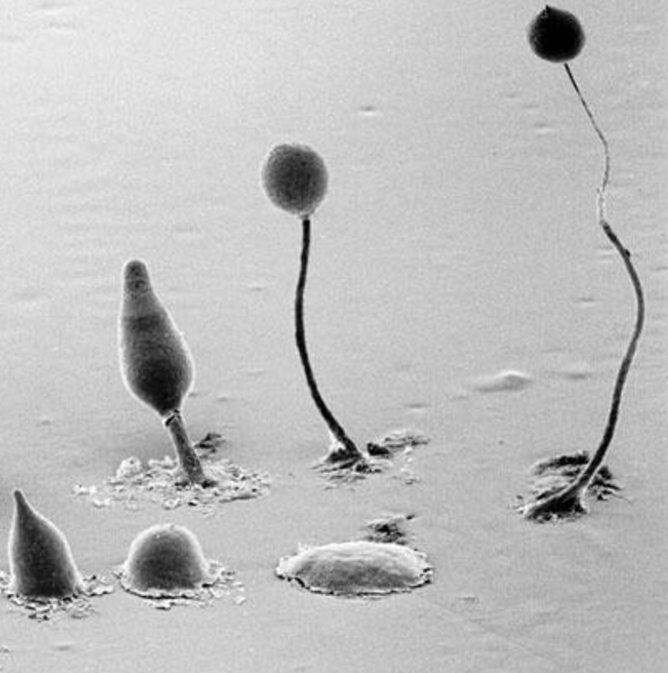
\includegraphics[width=0.9\columnwidth]{../2017-04-11_BAMC/Pics/socex_dictyostelium.pdf}\piccredit{Grimson \& Blanton}};

\node[thepic, anchor=west] at(\rad, \rad){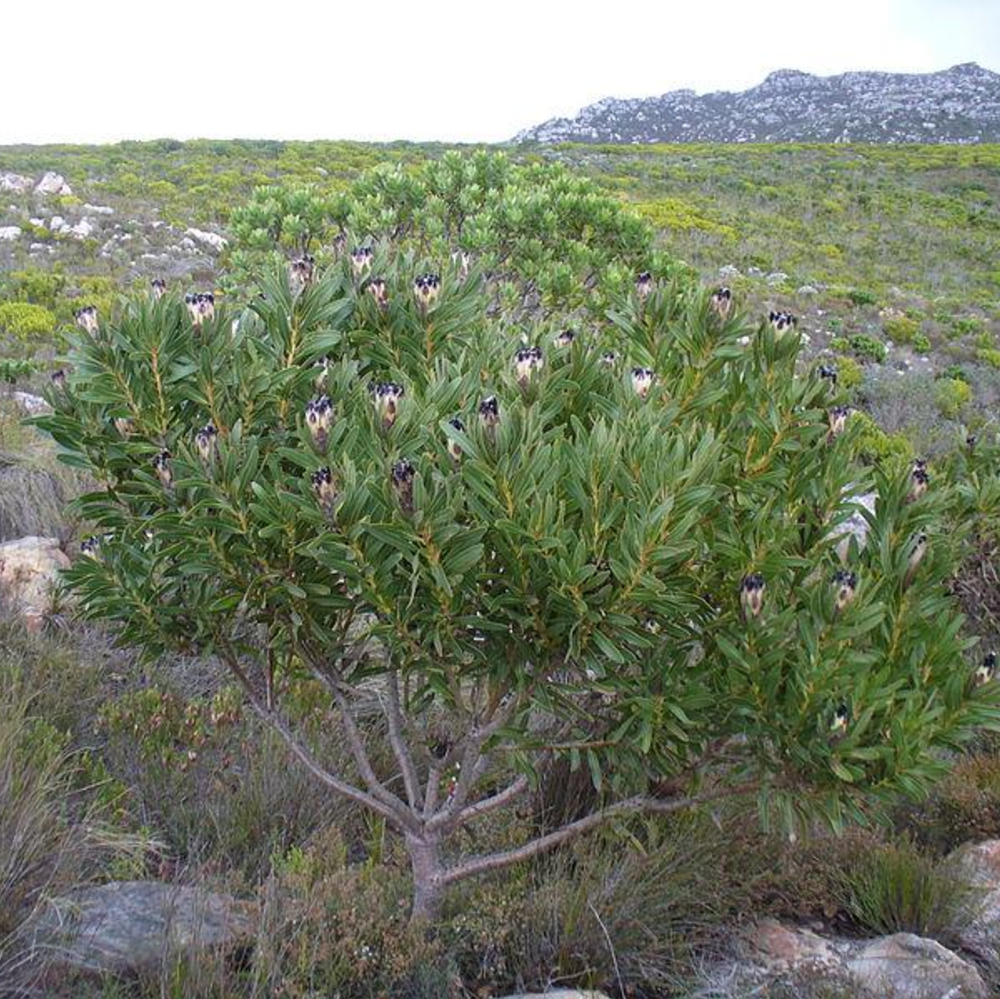
\includegraphics[width=0.9\columnwidth]{../2017-04-11_BAMC/Pics/socex_Protea_lepidocarpodendron.pdf}\piccredit{Wikimedia}
};

\node[thepic, anchor=east] at(-\rad, -\rad){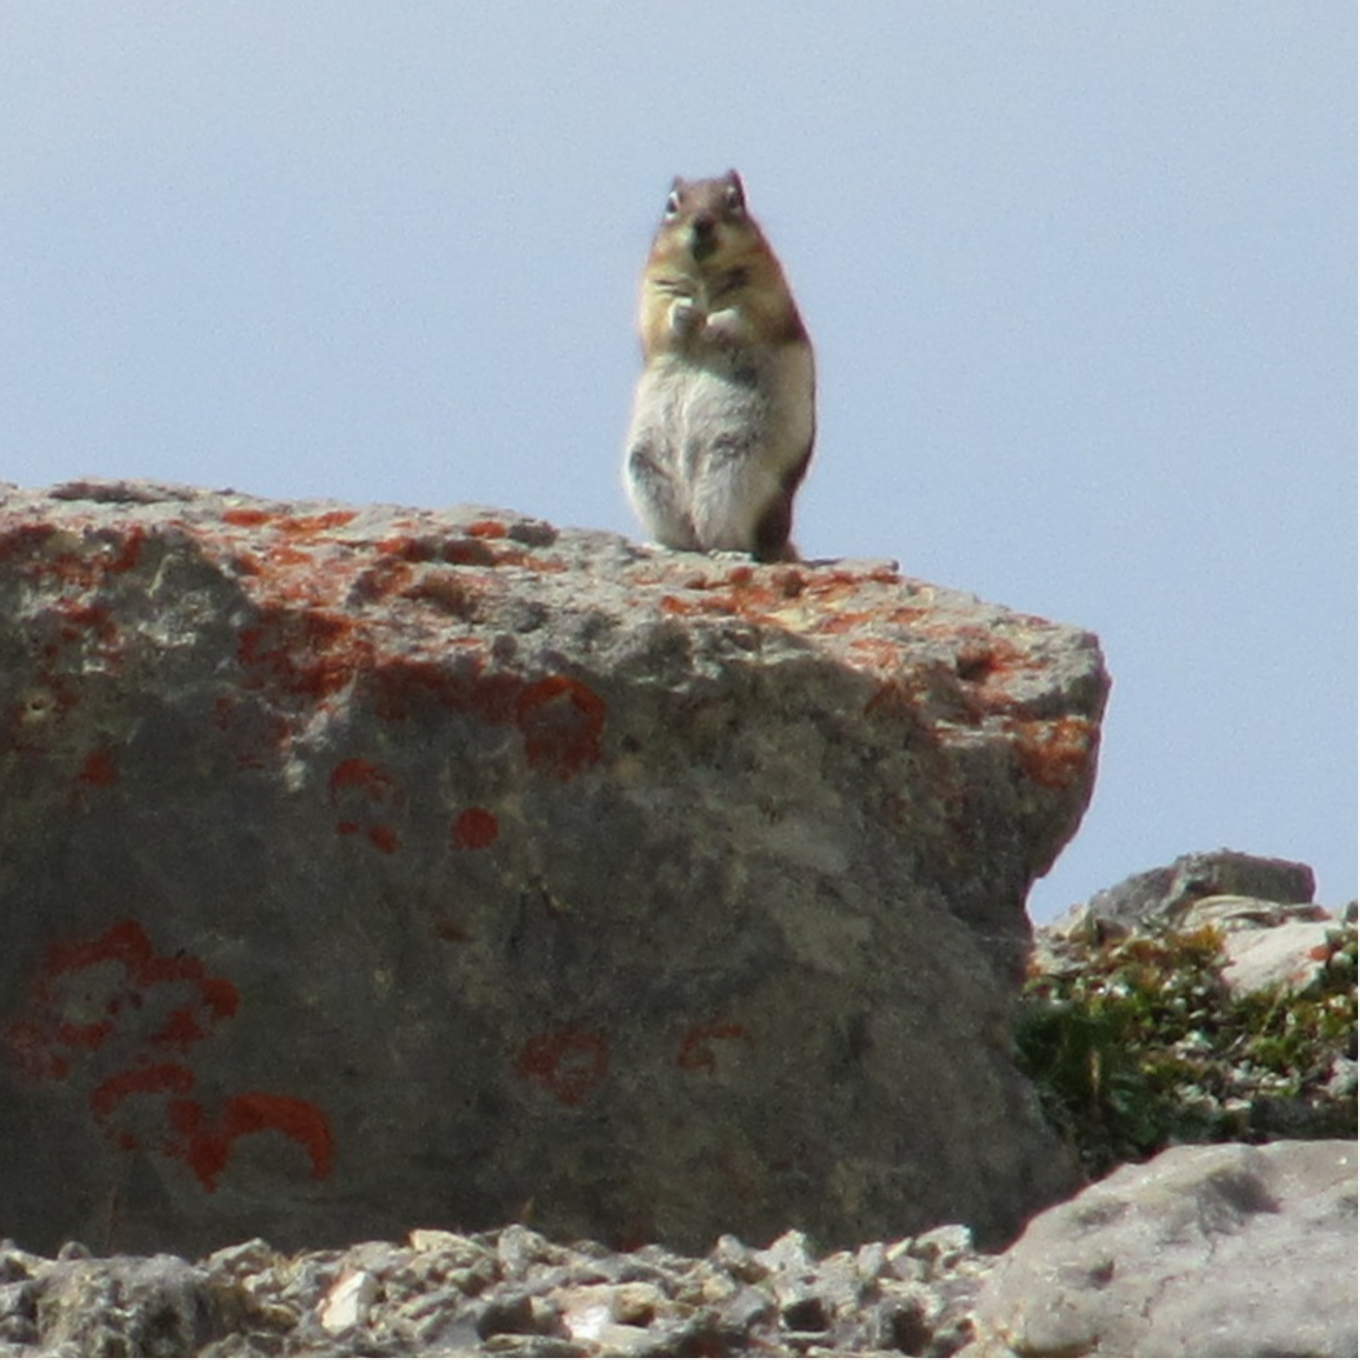
\includegraphics[width=0.9\columnwidth]{../2017-04-11_BAMC/Pics/socex_sentinelle.pdf}\piccredit{FD}
};

\node[thepic, anchor=west] at(\rad, -\rad){
\includegraphics[width=0.9\columnwidth]{../2017-04-11_BAMC/Pics/socex_superman.pdf}\piccredit{picturesforcoloring.com}
};
} % end examples uncover

\uncover<5>{
% Relatedness
\foreach \i in {1,...,6}{
\node[dck, circle, fill=white, draw=none] at (c\i){
\includegraphics[height=\hh]{../2016-07_ECMTB/Pics/typeA.pdf}};
} % end foreach 
} % end uncover

% Spatial structure
\uncover<6->{
\draw[lnk] (c1)--(c2)--(c3)--(c4)--(c5)--(c6)--(c1){};
\foreach \i in {2,3,4}{
\node[dck] (c3\i) at($(c3)+(\i*60:\rad)$){
\includegraphics[height=\hh]{../2016-07_ECMTB/Pics/type0.pdf}};
\draw[lnk] (c3)--(c3\i){};
\node[dck] (c6\i) at($(c6)+(\i*60-180:\rad)$){
\includegraphics[height=\hh]{../2016-07_ECMTB/Pics/type0.pdf}};
\draw[lnk] (c6)--(c6\i){};
}
\draw[lnk] (c2)--(c32)--(c33)--(c34)--(c4){};
\draw[lnk] (c1)--(c64)--(c63)--(c62)--(c5){};
}


\end{tikzpicture}
\end{center}
\end{frame}


\subsection{Subdivided populations}

\begin{frame}{\textcolor{gray}{Social evolution} in subdivided populations:\\ \textcolor{gray}{Beyond the usual assumptions}
}

\begin{tikzpicture}
\tikzstyle{popn}=[ellipse, draw=maincol, line width=1.5pt, inner sep = 0pt]
\tikzstyle{dck}=[inner sep=0pt, circle]
\def \rad {0.7cm}
\def \theduck {
\includegraphics[height=0.55cm]{../2016-07_ECMTB/Pics/type0.pdf}}

\node[dck]at(0,0) (d1){\theduck};
\foreach \i in {1,...,6}{
\node[dck] (d1\i) at($(d1)+(\i*60:\rad)$){\theduck};
}

\node[dck]at(3,3)(d2){\theduck};
\foreach \i in {1,...,4}{
\node[dck] (d2\i) at($(d2)+(\i*90:\rad)$){\theduck};
}

\node[dck]at(3.5, -1)(d3){\theduck};
\foreach \i in {1,...,8}{
\node[dck] (d3\i) at($(d3)+(\i*45:\rad)$){\theduck};
}

\node[dck]at(7,-0.7)(d4){\theduck};
\foreach \i in {1,...,6}{
\node[dck] (d4\i) at($(d4)+(\i*60:\rad)$){\theduck};
}

\node[dck]at(6.5,2.5)(d5){\theduck};
\node[dck] (d51) at($(d5)+(0:\rad)$){\theduck};

\uncover<2->{
% Add pop circles
\node[popn, fit=(d11)(d12)(d13)(d14)(d15)(d16)] (c1){};
\node[popn, fit=(d2)(d21)(d22)(d23)(d24)] (c2){};
\node[popn, fit=(d31)(d32)(d33)(d34)(d35)(d36)(d37)(d38)] (c3){};
\node[popn, fit=(d41)(d42)(d43)(d44)(d45)(d46)] (c4){};
\node[popn, fit=(d5)(d51)] (c5){};
}

\uncover<2->{
\tikzstyle{lnk}=[maincol, line width = 3pt, line cap=round]
\draw[lnk](c1)--(c2)--(c3)--(c1);
\draw[lnk](c2)--(c4)--(c5)--(c3)--(c4)--(c2);
\draw[lnk](c2)--(c5);
}

\end{tikzpicture}

\end{frame}

\subsection{Usual assumptions}
\begin{frame}{\textcolor<1-7>{gray}{Social evolution in subdivided populations:}\\ \textcolor<1-7>{gray}{Beyond }the usual assumptions}

\begin{columns}[c]
\begin{column}{0.55\textwidth} 
\begin{itemize}[<+-|alert@+>]
\item \sta<9>{Infinite population size}
\item Demes of equal sizes
\item Global dispersal
\item Constant population size
\item One trait under selection
\item Effects on fecundity
\item Weak selection
\item \sta<9>{Perfect strategy transmission}
\end{itemize}
\end{column}

\begin{column}{0.45\textwidth} 
\begin{center}

\only<1>{
{\Huge $\infty$}
\vspace{1em}

$\mathbb{E}[\,]$ vs. $\mathrm{Ave}(\,)$
}

\only<2,4>{\includegraphics[width=\columnwidth]{samedemesize.pdf}}

\only<3>{\includegraphics[width=\columnwidth]{globaldispersal.pdf}}

\only<5>{
\begin{tikzpicture}
\def \hh {1cm}
\node[](dA){
\includegraphics[height=\hh]{../2016-07_ECMTB/Pics/typeA.pdf}};

\node[right = of dA](dB){
\includegraphics[height=\hh]{../2016-07_ECMTB/Pics/typeB.pdf}};

%\node[below = of dA]{\includegraphics[height=\hh]{../2016-09_Fukuoka/Pics/duck_smallwings.pdf}};

%\node[below = of dB]{\includegraphics[height=\hh]{../2016-09_Fukuoka/Pics/duck_wings.pdf}};
\end{tikzpicture}
}

\only<6>{\includegraphics[height=1.5cm]{../GlobalPics/SocialEvol/bebe.pdf}}

\only<7>{
\begin{itemize}
\item[$\bullet$] Small contribution from the game \newline{\small ($w$-weak selection)}
\item[$\bullet$] Small phenotypic differences \newline{\small($\delta$-weak selection)}\newline
$\to$ Linearization
\end{itemize}



{\hspace{\stretch{1}} \footnotesize \pprref{Wild \& Traulsen}{2007}}
}

\only<8>{
\begin{tikzpicture}
\def \hh {1cm}
\node[](dA){
\includegraphics[height=\hh]{../2016-07_ECMTB/Pics/typeA.pdf}};
\node[right = of dA](dA2){
\includegraphics[height=\hh]{../2016-07_ECMTB/Pics/typeA.pdf}};

\node[below = of dA](dB){
\includegraphics[height=\hh]{../2016-07_ECMTB/Pics/typeB.pdf}};
\node[right = of dB](dB2){
\includegraphics[height=\hh]{../2016-07_ECMTB/Pics/typeB.pdf}};

\tikzstyle{toar}=[->, line width=1.5pt]
\draw[toar](dA)--(dA2);
\draw[toar](dB)--(dB2);
\end{tikzpicture}

}
\end{center}
\end{column}
\end{columns}
\end{frame}


\section{My work}
%% TITLE FRAME

\begin{frame}{}

\begin{center}
\begin{tikzpicture}
\def \hhh {0.5cm}
\def \dxx {0.15cm}
\node[inner sep=0pt](anc){};
\node[left= 0.5*\dxx of anc](lanr){\includegraphics[height=\hhh]{../GlobalPics/logo_anr.pdf}};
\node[left=\dxx of lanr](lcnrs){\includegraphics[height=\hhh]{../GlobalPics/logo_cnrs.pdf}};
\node[right= 0.5*\dxx of anc](lcdf){\includegraphics[height=\hhh]{../GlobalPics/logo_cdf.pdf}};
\node[right= \dxx of lcdf](lsmi){\includegraphics[height=\hhh]{../GlobalPics/logo_smile.pdf}};
\end{tikzpicture}

\btVFill

\begin{tikzpicture}
\node[text width=0.8\textwidth, font=\large, align=center, color=maincol](tit){Fidelity of parent-offspring transmission\\ and the evolution of social
\mbox{behavior} in subdivided populations.};

\tikzstyle{nameauthor}=[inner sep=2pt, draw=none, anchor=base]
\def \dhn {2.25cm}
\node[below=1cm of tit, nameauthor](FD){F. D\'ebarre};
%\path(SY.base)--(FG.base) node [pos=0.45, anchor=base]{\&};
\def \hsp{1cm}
\def \dsp {0.1cm}
\tikzstyle{spic}=[fill=gray40, circle, inner sep=-2.5pt]
%\node[spic, below=\dsp of FD](sFD){\includegraphics[height=\hsp]{../GlobalPics/SouthPark/SP_trp/sp_flo.pdf}};
\node[below=-0.35cm of FD](sFD){}; % Removing pic because looks odd with single author
\tikzstyle{twee}=[font=\footnotesize, minimum height=2em]
\node[below=0cm of sFD, twee](tFD){@flodebarre};
\node[left=0cm of tFD]{\includegraphics[height=1em]{../GlobalPics/twitter.pdf}};
\end{tikzpicture}

\vspace{1em}
{\footnotesize CNRS \\ Centre de Recherches Interdisciplinaires en Biologie, Paris}
\btVFill
MMEE, July 2017
\btVFill
\end{center}
\end{frame}

\subsection{Model}
\subsubsection{Mutation}
\begin{frame}{Fidelity of parent-offspring transmission}
\begin{columns}[b]
\begin{column}{0.7\textwidth}
\begin{block}{Causes of imperfect strategy transmission}
\begin{itemize}
\item<1-> Mutation
\item<2-> Partial heritability
\item<3-> Cultural transmission (vertical)
\end{itemize}
\end{block}
\end{column}
\begin{column}{0.25\textwidth}
\uncover<1->{\includegraphics[width=\columnwidth]{../2016-07_ECMTB/Pics/kylo.pdf}}
\end{column}
\end{columns}

\uncover<4->{
\begin{block}{In the model}
\begin{center}
	\begin{tikzpicture}
	\def \xdist {2.75cm}
	\def \ydist {0.8cm}
	\def \dydist {0.5cm}
	\def \hh {0.65cm}
	\tikzstyle{circindiv}=[text width=0.65cm, inner sep=0pt, align=center] % Circle for individual type
	\tikzstyle{lin}=[line width=2pt, >=angle 45, draw=ta3gray] % Line type
	\tikzstyle{arr}=[->, lin] % Arrow type, using line type
	\tikzstyle{arrlab}=[inner sep=3pt, draw=none] % Label on arrow
	\tikzstyle{labtt}=[draw=none] % Label/title
		
	\node[circindiv] at (0,0) (oo) {
\includegraphics[height=\hh]{../2016-07_ECMTB/Pics/type0.pdf}}; % Parent

\uncover<5->{
	\node[circindiv] at (\xdist, \ydist) (ono){
\includegraphics[height=\hh]{../2016-07_ECMTB/Pics/type0.pdf}}; % Unmutated offspring
	\draw[arr] (oo)--(ono) node [midway, above, sloped, arrlab] {$1-\mu$}; % Arrow between the two
}


\uncover<7->{
	\node[circindiv] at (\xdist, -\ydist+\dydist) (omutA){
\includegraphics[height=\hh]{../2016-07_ECMTB/Pics/typeA.pdf}}; % Mutation A
	\node[right=-0.cm of omutA, inner sep=0pt](labA) {A};

	\node[circindiv] at (\xdist, -\ydist-\dydist) (omutB){
\includegraphics[height=\hh]{../2016-07_ECMTB/Pics/typeB.pdf}}; % Mutation B
	\node[right=-0.cm of omutB, inner sep=0pt](labB) {B};
}

\uncover<5->{
	\node[labtt, anchor=south] at ($ (ono) + (0,0.75cm)$) (laboff){Offspring};
}
\uncover<4->{
	\node[labtt, anchor=base] at (oo |- laboff.base){Parent};
}

\uncover<6->{
	% Tmp node for the broken arrows
	\node[inner sep=0pt, minimum width=2pt, fill=ta3gray, circle] at (0.5*\xdist, -\ydist) (tmp)	{};
	\draw [lin] (oo)--node[midway, above, sloped, arrlab]{$\mu$} (tmp.center) ;
}

\uncover<7->{
	\draw [arr, line width=1.5pt] (tmp.center)--node[midway, above, sloped, arrlab]{$p$} (omutA) ;
	\draw [arr, line width=1.5pt] (tmp.base)--node[midway, below, sloped, arrlab]{$1-p$} (omutB) ;
}

\uncover<6->{
	\node [fit=(labA) (labB)] (fit) {};              
    \draw [decorate, line width=1pt, decoration={brace,mirror, amplitude=0.25cm}] (fit.south east) -- (fit.north east) node[midway, right, anchor=west, draw=none, xshift=0.25cm] (labmut) {Mutated};
}
    
    
    \uncover<5->{
    \node[anchor=west, draw=none] at (labmut.west |- ono){Unmutated};
}
    
\end{tikzpicture}
\end{center}

\end{block}
}

\end{frame}
\begin{frame}{Markovian model}
\begin{center}
{\large  \alt<2->{$t-1$}{$t$}}

\begin{tikzpicture}
\def \hh {0.65cm}
\tikzstyle{dck}=[inner sep=0pt, circle, text width=\hh, draw=none, align=center]
\tikzstyle{lnk}=[line width=1.5pt, draw=fgcol]

\node[dck](p1)at(0,0){};

\def \distrad {1.2cm}
\foreach \i in {2,...,5}{
\node[dck](p\i)at($(p1)+(\i*90:\distrad)$){};
}

\def \xx {4}
\node[dck](p6) at(\xx, 0){};
\foreach \i in {7,...,10}{
\node[dck](p\i)at($(p6)+(\i*90:\distrad)$){};
}


% 0 ducks at time t
\uncover<1>{
\foreach \i in {1, ..., 10}{
\node[dck, draw=none]at(p\i) (d\i){
\includegraphics[width=\columnwidth]{../2016-07_ECMTB/Pics/type0.pdf}};
}
}

% Pops
\tikzstyle{popn}=[draw=maincol, line width = 1.5pt, circle, inner sep=0pt, minimum width = 3.75cm]

\node[popn](c1) at(0,0){};
\node[popn](c2) at(\xx,0){};


%  Ducks at time t-1
\uncover<2->{
\foreach \i in {1,2,4,5,7,8,10}{
\node[dck, draw=none]at(p\i) (d\i){
\includegraphics[width=\columnwidth]{../2016-07_ECMTB/Pics/typeA.pdf}};
}

\foreach \i in {3, 6, 9}{
\node[dck, draw=none]at(p\i) (d\i){
\includegraphics[width=\columnwidth]{../2016-07_ECMTB/Pics/typeB.pdf}};
}

} % end uncover

% 
\includegraphics[height=\columnwidth]{../2016-07_ECMTB/Pics/typeA.pdf}
\end{tikzpicture}
$\mathbb{E}[\overline{X}(t)] $\uncover<2->{$= \mathbb{E}[\mathbb{E}[\overline{X}(t)| X(t-1)]]$}
\end{center}
The frequency of altruists in the population at a given time\uncover<2->{ depends on the \textbf{\alert{state}} of the population at the previous time step.}
\end{frame}




\begin{frame}{Genealogy, Identity by descent and Identity in state}
\begin{center}
\begin{tikzpicture}
\def \nlines {5}
\def \ncols {10}
\def \dx {0.7cm}
\def \dy {0.9cm}
\tikzstyle{indivbase}=[circle, inner sep=0pt, text width=0.5cm, fill=bgcol, draw=none]
\tikzstyle{genlink}=[draw=fgcol, line width=1.2pt]
\foreach \i in {1,...,\nlines}{
\foreach \j in {1,...,\ncols}{
	\node[indivbase] at(\dx*\j, -\dy*\i) (c\i\j) {};
}}

\uncover<1->{
\foreach \i in {1,...,\nlines}{
\foreach \j in {1,...,\ncols}{
	\node[indivbase, draw=fgcol] at(c\i\j) {};
}}
}

\draw[->, >=angle 45] (-0.5*\dx, 0)--(-0.5*\dx, -\nlines*\dy-\dy){} node [above, anchor=north east] {Time};

\tikzstyle{iA}=[indivbase, fill=colA]
\tikzstyle{iB}=[indivbase, fill=colB]

% Genealogy
\tikzstyle{mut}=[color=tascarletred, font=\small]
\newcommand{\symbmut}{$\bigstar$}

\uncover<2->{
\draw[genlink] (c11)--(c21);
\draw[genlink] (c11)--(c22);
\draw[genlink] (c11)--(c23);
\draw[genlink] (c13)--(c24);
\draw[genlink] (c15)--(c25);
\draw[genlink] (c17)--(c26);
\draw[genlink] (c17)--(c27);
\draw[genlink] (c17)--(c28);
\draw[genlink] (c110)--(c29);
\draw[genlink] (c110)--(c210);

\draw[genlink] (c21)--(c31);
\draw[genlink] (c21)--(c32);
\draw[genlink] (c24)--(c33);
\draw[genlink] (c25)--(c34);
\draw[genlink] (c25)--(c35);
\draw[genlink] (c26)--(c36);
\draw[genlink] (c27)--(c37);
\draw[genlink] (c28)--(c38);
\draw[genlink] (c29)--(c39);
\draw[genlink] (c29)--(c310);

\draw[genlink] (c32)--(c41);
\draw[genlink] (c32)--(c42);
\draw[genlink] (c32)--(c43);
\draw[genlink] (c35)--(c44);
\draw[genlink] (c36)--(c45);
\draw[genlink] (c36)--(c46);
\draw[genlink] (c38)--(c47);
\draw[genlink] (c38)--(c48);
\draw[genlink] (c39)--(c49);
\draw[genlink] (c310)--(c410);

\draw[genlink] (c42)--(c51);
\draw[genlink] (c42)--(c52);
\draw[genlink] (c43)--(c53);
\draw[genlink] (c45)--(c54);
\draw[genlink] (c45)--(c55);
\draw[genlink] (c46)--(c56);
\draw[genlink] (c47)--(c57);
\draw[genlink] (c47)--(c58);
\draw[genlink] (c48)--(c59);
\draw[genlink] (c48)--(c510);
}

\uncover<3->{
\node[iA] at (c11){};
\node[iA] at (c12){};
\node[iA] at (c13){};
\node[iA] at (c14){};
\node[iA] at (c15){};
\node[iA] at (c16){};
\node[iB] at (c17){};
\node[iA] at (c18){};
\node[iA] at (c19){};
\node[iA] at (c110){};
}

\uncover<4->{
\node[iA] at (c21){};
\node[iA] at (c22){};
\node[iA] at (c23){};
\node[iA] at (c24){};
\node[iA] at (c25){};
\node[iB] at (c26){};
\node[iB] at (c27){};
\node[iB] at (c28){};
\node[iA] at (c29){};
\node[iA] at (c210){};

\node[iA] at (c31){};
\node[iA] at (c32){};
\node[iA] at (c33){};
\node[iA] at (c34){};
\node[iA] at (c35){};
\node[iB] at (c36){};
\node[iB] at (c37){};
\node[iB] at (c38){};
\node[iA] at (c39){};
\node[iA] at (c310){};

\node[iA] at (c41){};
\node[iA] at (c42){};
\node[iA] at (c43){};
\node[iA] at (c44){};
\node[iB] at (c45){};
\node[iB] at (c46){};
\node[iB] at (c47){};
\node[iB] at (c48){};
\node[iA] at (c49){};
\node[iA] at (c410){};

\node[iA] at (c51){};
\node[iA] at (c52){};
\node[iA] at (c53){};
\node[iB] at (c54){};
\node[iB] at (c55){};
\node[iB] at (c56){};
\node[iB] at (c57){};
\node[iB] at (c58){};
\node[iB] at (c59){};
\node[iB] at (c510){};

}

\uncover<5->{
\path(c11)--(c21) node[midway, mut]{\symbmut};
\node[iB] at (c31){};
\node[iB] at (c32){};
\node[iB] at (c41){};
\node[iB] at (c42){};
\node[iB] at (c43){};
\node[iB] at (c51){};
\node[iB] at (c52){};

\path(c26)--(c36) node[midway, mut]{\symbmut};
\node[iA] at (c36){};
\node[iA] at (c46){};
\node[iA] at (c45){};
\node[iA] at (c54){};
\node[iA] at (c55){};
\node[iA] at (c56){};

\path(c43)--(c53) node[midway, mut]{\symbmut};
}

\tikzstyle{pairexamples}=[rectangle, rounded corners, draw=maincol, inner sep=2pt, line width=1pt]
\uncover<6>{
\node[fit=(c53)(c54), pairexamples]{};
}
\uncover<7>{
\node[fit=(c53)(c52), pairexamples]{};
}
\uncover<8>{
\node[fit=(c54)(c55), pairexamples]{};
}

\end{tikzpicture}
\end{center}

\end{frame}

\begin{frame}{Expected state of pairs of sites and identity by descent}

At neutrality (i.e., in the absence of selection, $\delta = 0$),
\vspace{1em}

\begin{center}

\uncover<2->{
\begin{tikzpicture}
\tikzstyle{eqpart}=[rectangle, draw=none, inner sep=1pt, minimum height=0.55cm, rounded corners, font=\Large]
\tikzstyle{expl}=[rectangle, inner sep=2pt, draw=none, align=left, font=\small]
\tikzstyle{arrexp}=[->, >=stealth, line width=1.2pt, draw=gray]

\def \dye {0.4cm}
\node[eqpart](Pij){$P_{ij}$};
\node[expl, below=\dye of Pij.south east, anchor=north east, align=right, text width=4.cm](eP){Expected state of the $i,j$ pair\\= Probability that the two individuals are altruists};

\draw[arrexp](Pij.south)--(eP);

\def \dx {0.25cm}
\uncover<3->{
\node[eqpart, right= \dx of Pij](equal){$=$};

\node[eqpart, right= \dx of equal](rhs1){$Q_{ij}$};
\node[eqpart, right= 0 of rhs1](rhs2){$ p $};

\node[expl, anchor=north, text width=6.5cm, align=center] at ($(rhs1 |- eP.south east)+(0,-\dye)$) (e1){Probability that the individuals at sites $i$ and $j$ are identical by descent \\ (no mutation since their common ancestor)};
\draw[arrexp](rhs1)--(e1);
}
\uncover<4->{
\node[expl, anchor=west, text width=4.5cm] at ($(rhs2|-eP)+(-0.cm,0)$)(e2){Probability that a mutant is an altruist \\= Probability that a given site is occupied by an altruist};
\draw[arrexp](rhs2.south)--(e2);
}

\uncover<5->{
\node[eqpart, right= 0 of rhs2](rhs3){$ + $};
\node[eqpart, right= 0 of rhs3](rhs4){$ (1-Q_{ij}) p^2$};
}


\end{tikzpicture}
} % end uncover
\end{center}
\uncover<6>{
{
\Large
\begin{center}
$Q_{\textsf{in}}$, $Q_{\textsf{out}}$
\end{center}
}
}
\end{frame}

\subsubsection{Updating rules}
\begin{frame}{Life-cycles / Updating rules}

\pause
{
\begin{block}{Generic}
\begin{description}
\item<+->[$B_{ij}$] Probability that individual at site $j$ has offspring at site $i$ at the next time step
\item<+->[$D_j$] Probability that the individual at site $j$ has died at the next time step.
\end{description}
\uncover<+->{
Both depend on the state of the population ($X$).
}
\end{block}

\begin{block}<+->{Specific}
\def \hh {1.2em}
\begin{tabular}{p{0.3\linewidth}p{0.3\linewidth}p{0.3\linewidth}}
\multicolumn{2}{c}{Moran} & Wright-Fisher\\
Birth-death & Death-birth &  %\\ \hline \tiny &\tiny & \tiny 
\\
\Large 1 \includegraphics[height=\hh]{../GlobalPics/SocialEvol/bebe.pdf}, \newline
1 \includegraphics[height=\hh]{../GlobalPics/SocialEvol/tombstone.pdf}
&
\Large 1 \includegraphics[height=\hh]{../GlobalPics/SocialEvol/tombstone.pdf}, \newline
1 \includegraphics[height=\hh]{../GlobalPics/SocialEvol/bebe.pdf}
&
 \Large $N$ \includegraphics[height=\hh]{../GlobalPics/SocialEvol/bebe.pdf} {\normalsize and} 
$N$ \includegraphics[height=\hh]{../GlobalPics/SocialEvol/tombstone.pdf} \\ 
$\sum_{j=1}^N D_j = 1$
&
$D_j=1/N$
&
$D_j = 1$.
\end{tabular}
\end{block}
}

\end{frame}


\subsubsection{Effects of interactions}


\begin{frame}{Effects of social interactions}
\begin{itemize}[<+->]
\item Social interactions affect \alert{fecundity} (could also affect survival)
\item Individual fecundity depends on the state of the population \\($N$ potential interactants and focal individual itself). \alert{Generically},
\begin{displaymath}
f_i(X,\delta) = F_i \left(e_{1i} \delta X_1, \dots, e_{li} \delta X_l, \dots, e_{Ni} \delta X_N; \delta X_i\right);
\end{displaymath}
\end{itemize}
%
%
\vspace{-2ex}
\begin{block}<+->{Weak selection ($\delta  \ll 1$)}
Assuming a baseline fecundity of $1$, at the first order we obtain
\begin{displaymath}
f_i(X,\delta) = 1 + \delta \left(\mathsf{b} \sum_{l=1}^N e_{li} X_l  - \mathsf{c} X_i \right) + O(\delta^2). 
\end{displaymath}
\vspace{-1em}
\uncover<+->{\small
\begin{displaymath}
M = \begin{array}{cccc}
 && \multicolumn{2}{c}{\textsf{\footnotesize Donnors}}\\
 && 
\includegraphics[width=0.3cm]{../2016-07_ECMTB/Pics/typeA.pdf} & 
\includegraphics[width=0.3cm]{../2016-07_ECMTB/Pics/typeB.pdf} \\
\multirow{2}{*}{\rotatebox[origin=c]{90}{\textsf{\footnotesize Recipients}}}& \vcenter{\hbox{
\includegraphics[width=0.3cm]{../2016-07_ECMTB/Pics/typeA.pdf}}} & b - c &  -c \\ \\
%
& \vcenter{\hbox{\includegraphics[width=0.3cm]{../2016-07_ECMTB/Pics/typeB.pdf}}} & b & 0\\
\end{array}
\end{displaymath}
}
\end{block}
\end{frame}



\subsection{Results}
\subsubsection{Direct effects}
\begin{frame}{Expected frequency of altruists in the population}

\vspace{-1em}
\begin{displaymath}
\mathbb{E}[\overline{X}] \approx p + \delta \frac{p (1-p)}{\mu}  \left[ \bb \left( \alert<2>{\beta_D} - \beta_I \right) - \cc \left( \alert<2>{\gamma_D} - \gamma_I \right) \right]
\end{displaymath}

\pause
\begin{block}{Direct effects}
Moran BD, Moran DB, Wright-Fisher:
\begin{align*}
\beta_D & = (1-\mu) \alert<3>{Q_{\mathsf{in}}} \\
\gamma_D & = 1-\mu.
\end{align*}

\vspace{-1.5em}

\pause
\begin{center}
\small
\begin{tabular}{cc}
Moran & Wright-Fisher \vspace{-0.5em} \\ 
\includegraphics[width=0.4\textwidth]{Pics/QplotM.pdf}
&
\includegraphics[width=0.4\textwidth]{Pics/QplotWF.pdf}
\end{tabular}
\end{center}
\end{block}
\end{frame}


\subsubsection{Indirect Effects}
\begin{frame}{Expected frequency of altruists in the population [2]}
\vspace{-1em}
\begin{displaymath}
\mathbb{E}[\overline{X}] \approx p + \delta \frac{p (1-p)}{\mu}  \left[ \bb \left( \alert<2>{\beta_D} - \beta_I \right) - \cc \left( \alert<2>{\gamma_D} - \gamma_I \right) \right]
\end{displaymath}


\def \Moran {\mathsf{M}}
\def \BD {\mathsf{BD}}
\def \indirect {I}
\def \direct {D}
\def \Qin {Q_{\mathsf{in}}}
\def \Qout {Q_{\mathsf{out}}}
\def \DB {\mathsf{DB}}
\def \WF {\mathsf{WF}}

\pause
\begin{block}{Moran, Birth-Death}
{\footnotesize
\begin{displaymath}
\begin{split}
\beta_{\indirect}^{\BD} &=  (1-m) \left(\frac{n-1}{n} \Qin^{\Moran} + \frac{1}{n}\right) + m \, \Qout^{\Moran} %
- \mu \frac{ 1 + (n-1) \Qin^{\Moran} + n (d-1) \Qout^{\Moran}}{n d} = \gamma_{\indirect}^{\BD}.
\end{split}
\end{displaymath}
}
\end{block}

\begin{block}{\alt<3>{Wright-Fisher}{Moran, Death-Birth}}
{\footnotesize
\begin{displaymath}
\begin{split}
\beta_{\indirect}^{\DB} & = (1-\mu ) \Bigg[ \left( \frac{1}{n} + \frac{ (n-1) \Qin^{\alt<3>{\WF}{\Moran}} }{n} \right) \left( (1-m)^2 +  \frac{m^2}{ (d-1)} \right) \\ 
%
& \qquad \qquad \quad + m \, \left(2  (1-m) +  (d-2) \frac{m}{(d-1)}\right) \Qout^{\alt<3>{\WF}{\Moran}} \Bigg]  = \gamma_{\indirect}^{\DB}
%
\end{split}
\end{displaymath}
}
\end{block}
\uncover<3>{\phantom{i}}

\end{frame}

\subsubsection{Plots}
\def \wpic {3.5cm}

\begin{frame}{Expected frequency of altruists in the population [3]}

\begin{center}
\begin{tabular}{ccc}
Moran, Birth-Death & Moran, Death-Birth & Wright-Fisher\\
\includegraphics[width=\wpic, ]{Pics/{EXBD_sel0.005_htg0}.pdf}
&
\includegraphics[width=\wpic, ]{Pics/{EXDB_sel0.005_htg0}.pdf}
&
\includegraphics[width=\wpic, ]{Pics/{EXWF_sel0.005_htg0}.pdf}
\end{tabular}

\vspace{1em}
\textcolor{cl1}{$\mu=0.005$}, \textcolor{cl2}{$\mu = 0.010$}, \textcolor{cl3}{$\mu = 0.100$}, \textcolor{cl4}{$\mu = 0.250$}. 
\end{center}
\end{frame}

\subsubsection{Robustness}
\begin{frame}{Under strong selection {\normalsize($\delta = 0.1$; weak selection was $\delta = 0.005$)} }

\pause
\begin{center}
\begin{tabular}{ccc}
Moran, Birth-Death & Moran, Death-Birth & Wright-Fisher\\
\includegraphics[width=\wpic, ]{Pics/{EXBD_sel0.1_htg0}.pdf}
&
\includegraphics[width=\wpic, ]{Pics/{EXDB_sel0.1_htg0}.pdf}
&
\includegraphics[width=\wpic, ]{Pics/{EXWF_sel0.1_htg0}.pdf}
\end{tabular}

\vspace{1em}
\textcolor{cl1}{$\mu=0.005$}, \textcolor{cl2}{$\mu = 0.010$}, \textcolor{cl3}{$\mu = 0.100$}, \textcolor{cl4}{$\mu = 0.250$}. 
\end{center}
\end{frame}

\begin{frame}{Heterogeneous deme sizes ($\overline{n} = 4$ as before, but $1\leq n \leq 5$)}

\pause
\begin{center}
\begin{tabular}{ccc}
Moran, Birth-Death & Moran, Death-Birth & Wright-Fisher\\
\includegraphics[width=\wpic, ]{Pics/{EXBD_sel0.005_htg1}.pdf}
&
\includegraphics[width=\wpic, ]{Pics/{EXDB_sel0.005_htg1}.pdf}
&
\includegraphics[width=\wpic, ]{Pics/{EXWF_sel0.005_htg1}.pdf}
\end{tabular}

\vspace{1em}
\textcolor{cl1}{$\mu=0.005$}, \textcolor{cl2}{$\mu = 0.010$}, \textcolor{cl3}{$\mu = 0.100$}, \textcolor{cl4}{$\mu = 0.250$}. 
\end{center}
\end{frame}

\begin{frame}{With empty sites}

\begin{center}
\begin{tabular}{cc}
Density & Frequency \\
\includegraphics[width=\wpic]{Pics/{Emptysites_0.05_15_0.1_0_dens}.pdf}
&
\includegraphics[width=\wpic]{Pics/{Emptysites_0.05_15_0.1_0_freq}.pdf}
\end{tabular}
\end{center}

\end{frame}

\begin{frame}{Take-Home messages}

\begin{itemize}
\item<+-> Under weak selection (small phenotype differences, $\delta \ll 1$), it is possible to compute the expected frequency of social individuals, for
\begin{itemize}
\item any life-cycle \textcolor{gray}{(such that population size = $N$)}
\item any regular population structure \textcolor{gray}{(such that neutral reproductive values are equal to $1/N$)}
\item any mutation probability;
\end{itemize}
\item<+-> $\mathbb{E}[\overline{X}] > 0 \Leftrightarrow b \kappa > c$, \hspace{1ex} and $\kappa$ depends on 
\begin{itemize}
\item population structure,
\item life-cycle,
\item mutation.
\end{itemize}
\item<+-> In subdivided populations, $\mathbb{E}[X]$ can increase with the emigration probability $m$ when strategy transmission is imperfect ($\mu > 0$).
\item<+-> This result seems to hold under stronger selection and in heterogeneous populations.
\end{itemize}
\pause
\begin{center}
\textcolor{maincol}{Thanks for your attention!}
\end{center}
\end{frame}
\end{document}
